\bigbreak
\subsection*{Što je SoftEther VPN?}

\begin{wrapfigure}{r}{0.5\textwidth} 
     \centering
     
\includegraphics[width=0.5\textwidth]{SoftEther/SoftEtherLogo}
	\caption{Službeni logo SoftEther VPN-a}
\end{wrapfigure}
\hspace{0.5cm}
SoftEther VPN\cite{softether} besplatan je višeplatformski program otvorenog koda koji podržava korištenje različitih VPN protokola. Program je nastao 2013. godine kao akademski projekt na sveučilištu u Tsukubi i podržan je na različitim operacijskim sustavima kao što su Linux, FreeBSD, Mac, Solaris i Windows za koji je u ovom poglavlju prikazan postupak postavljanja i uporabe.
\smallbreak
Program SoftEther otvorenog je koda pa ga može bilo tko koristiti za vlastite ili komercijalne svrhe.\smallbreak
SoftEther VPN koristi HTTPS preko SSL (Secure Sockets Layer)\cite{ssl}
protokola kako bi omogućio siguran prijenos kriptiranih podataka preko Interneta. Uz njega su podržani unutar programa i ostali poznatiji protokoli kao što su OpenVpn, IPsec, L2TP, ...\\
Unutar programa sve postavke detaljno su objašnjene i mogu se podesiti korištenjem grafičkog sučelja što ovaj program čini jednostavnim za uporabu.

\FloatBarrier

\bigbreak
\subsection*{Instalacija SoftEther servera}
\hspace{0.5cm}
Za početak potrebno je preuzeti instalaciju VPN servera sa službene stranice SoftEthera:\\ \url{https://www.softether.org}
\begin{figure}[h!]
	\centering
     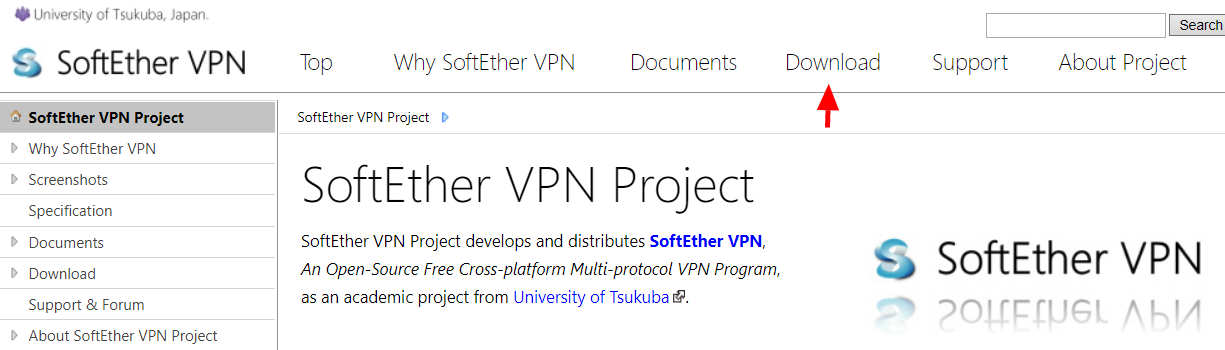
\includegraphics[width=0.6\textwidth]{SoftEther/korak1}
\end{figure}
\FloatBarrier
Odabirom ``Download'' iz izborne trake prikazuje se stranica s ponuđenim poveznicama za preuzimanje.
\begin{figure}[h!]
     \centering
     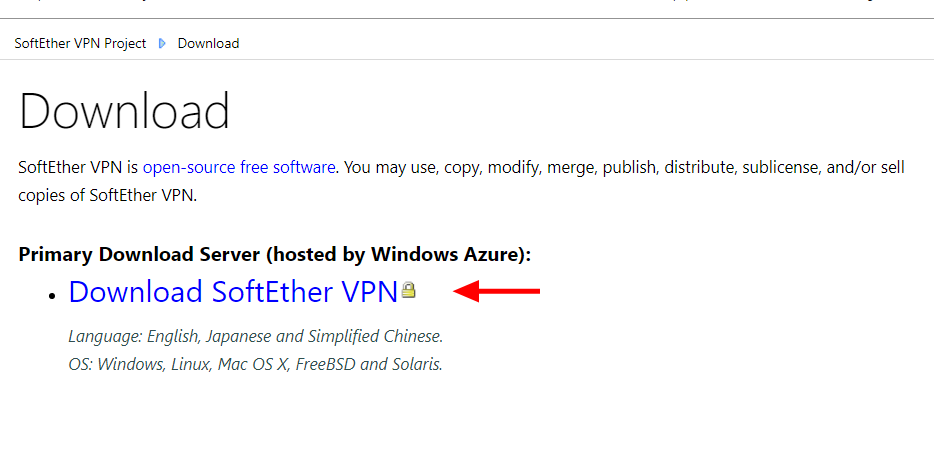
\includegraphics[width=0.6\textwidth]{SoftEther/korak2}
\end{figure}
\FloatBarrier
Sljedeći isječak prikazuje stranicu koja se otvori odabirom prve poveznice. Na stranici se nalaze izborni okviri u kojima je potrebno odabrati željeni program. Za preuzimanje VPN servera potrebno je odabrati postavke prikazane na sljedećem isječku te odabrati prvu poveznicu za početak preuzimanja.
\begin{figure}[h!]
     \centering
     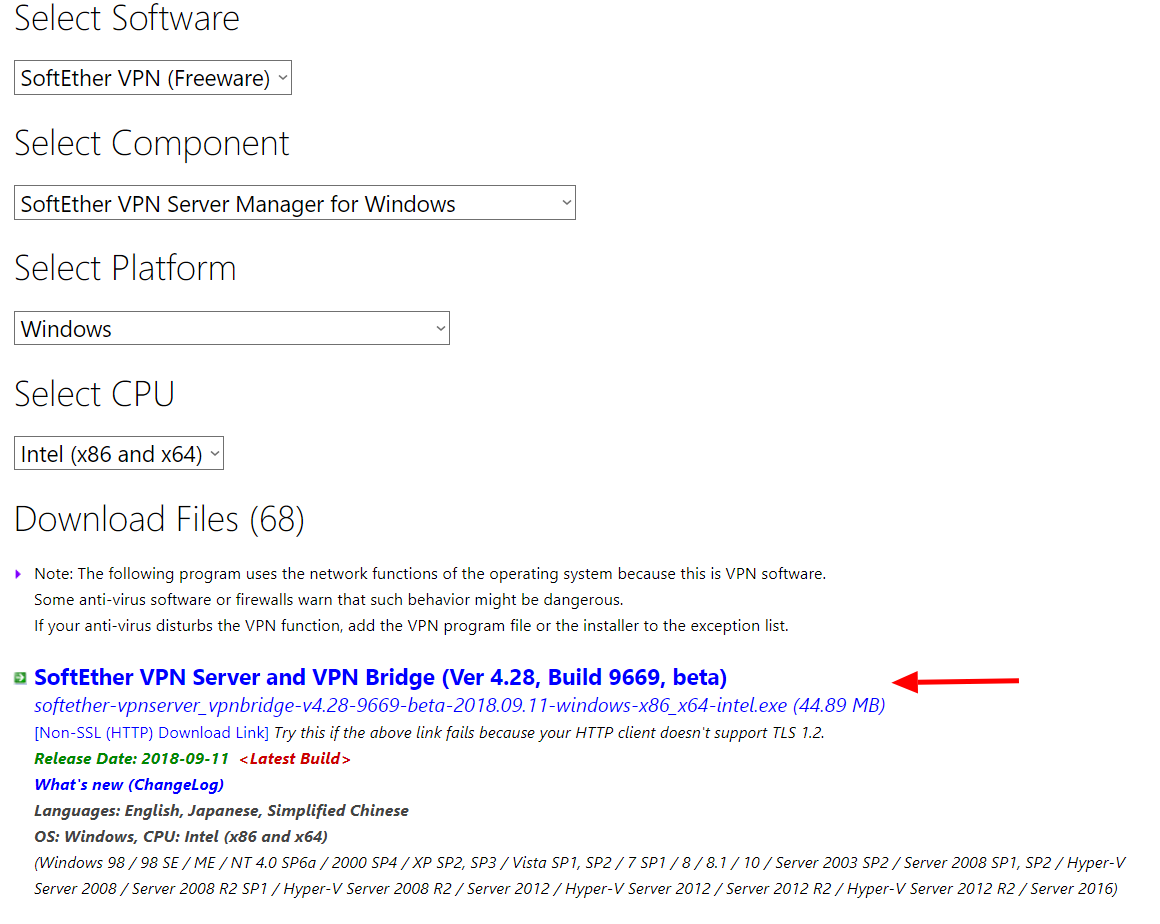
\includegraphics[width=0.6\textwidth]{SoftEther/korak6}
\end{figure}
\FloatBarrier
Nakon preuzimanja i pokretanja instalacije otvara se sljedeći prozor u kojemu se predlaže odabir prvog ponuđenog jer nudi potpunu instalaciju.
\begin{figure}[h!]
     \centering
     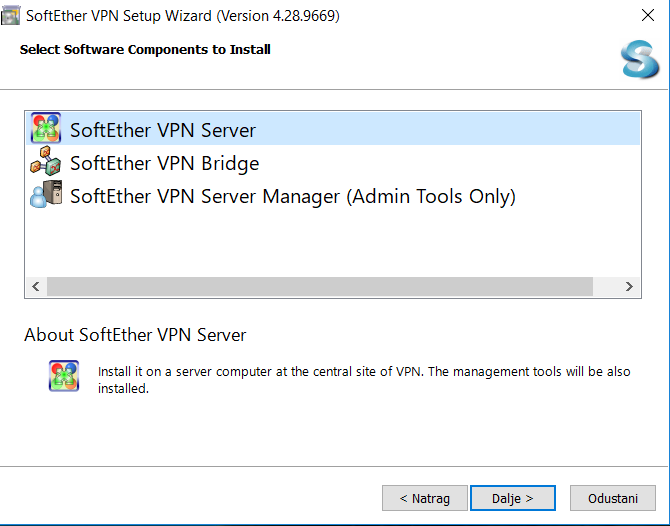
\includegraphics[width=0.6\textwidth]{SoftEther/korak7}
\end{figure}
\FloatBarrier
Nakon uspješne instalacije prikazuje se sljedeći okvir u kojem još nema niti jednog servera. Dodavanje servera započinje se odabirom ``New Setting''.
\begin{figure}[h!]
     \centering
     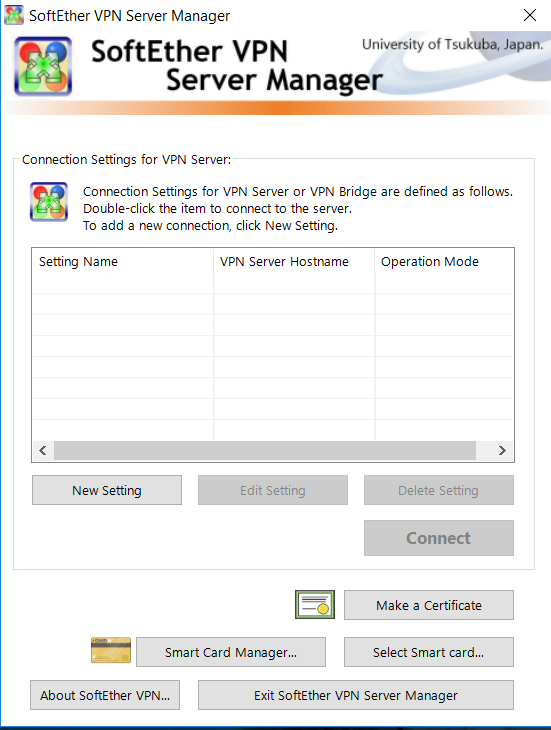
\includegraphics[width=0.6\textwidth]{SoftEther/korak8}
\end{figure}
\FloatBarrier
Stvaranje servera započinje se upisom željenog naziva u polje ``setting name'' i upisom vlastite IP adrese preko koje je trenutno računalo spojeno na Internet. Upute za pronalazak IP adrese mogu se pronaći na kraju ovog poglavlja. Preporuka je dodati lozinku za pristup serveru radi dodatne sigurnosti u polje ``password''.
\begin{figure}[h!]
     \centering
     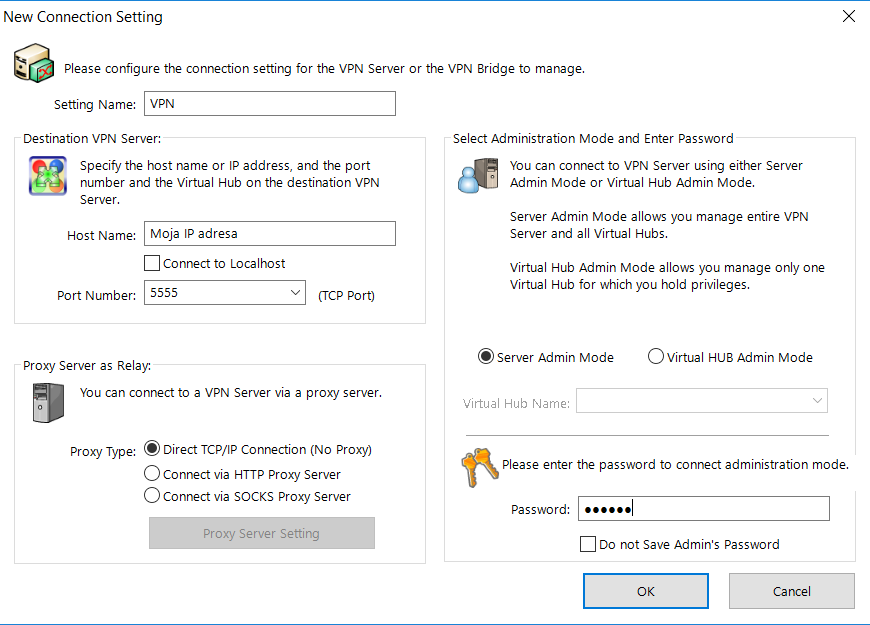
\includegraphics[width=0.6\textwidth]{SoftEther/korak9}
\end{figure}
\FloatBarrier
U tablici sada vidimo da je dodan novi server kojeg je potrebno konfigurirati odabirom ``Connect'' opcije.
\begin{figure}[h!]
     \centering
     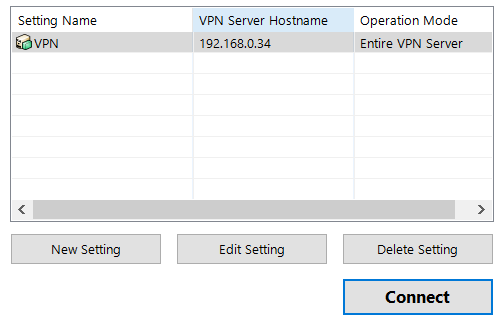
\includegraphics[width=0.6\textwidth]{SoftEther/korak10}
\end{figure}
\FloatBarrier
Kako bi se druga računala uspjela povezati s napravljenim serverom, potrebno je dodati virtualno čvorište odabirom opcije ``Create a Virtual Hub''.
\begin{figure}[h!]
     \centering
     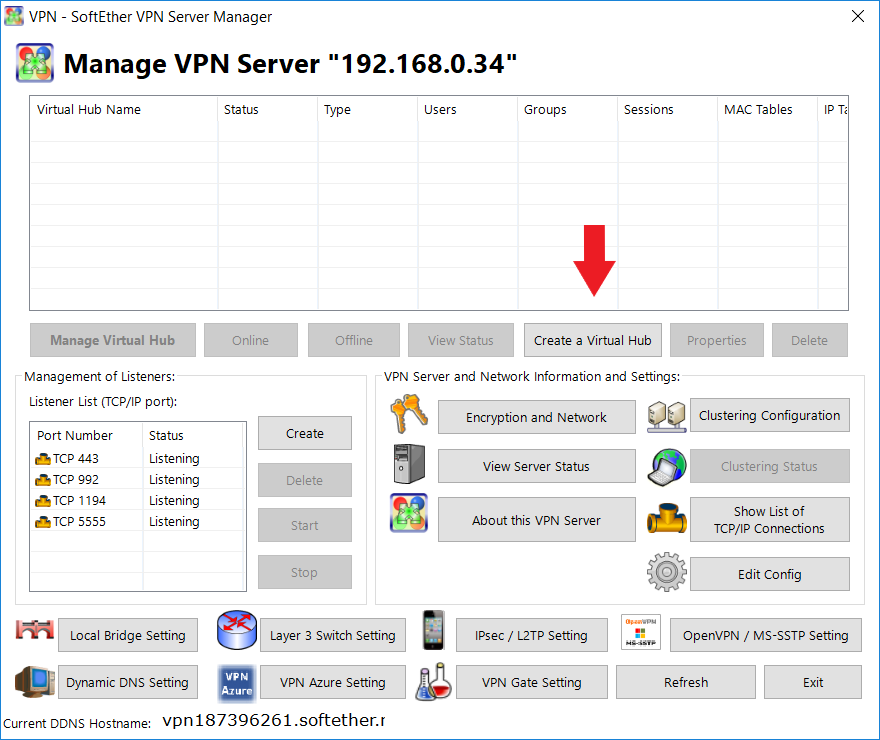
\includegraphics[width=0.6\textwidth]{SoftEther/korak11}
\end{figure}
\FloatBarrier
Virtualnom čvorištu postavljamo proizvoljno ime te dodajemo lozinku radi dodatne sigurnosti.
\begin{figure}[h!]
     \centering
     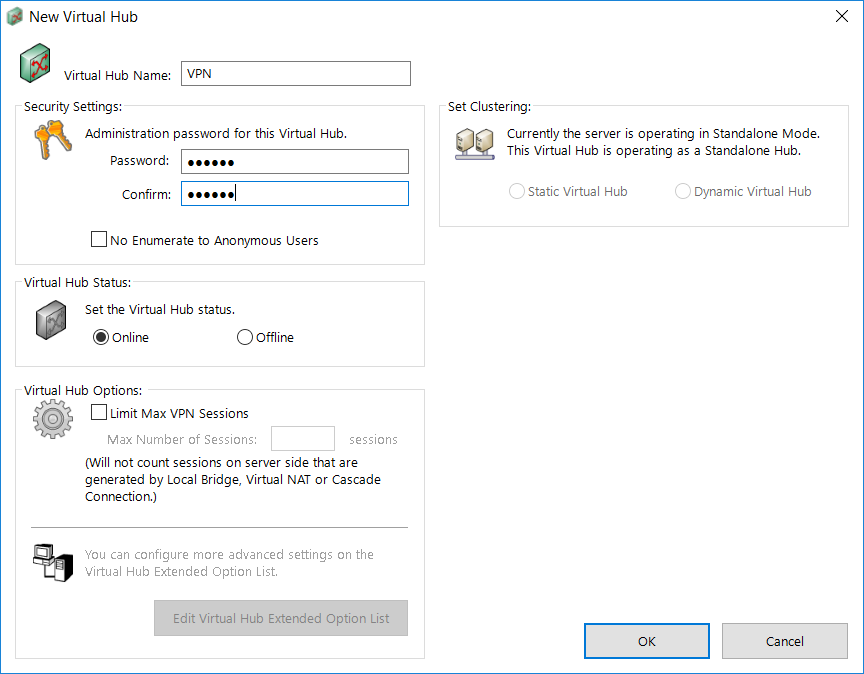
\includegraphics[width=0.6\textwidth]{SoftEther/korak12}
\end{figure}
\FloatBarrier
Sada se može vidjeti novo dodano čvorište u tablici.
\begin{figure}[h!]
     \centering
     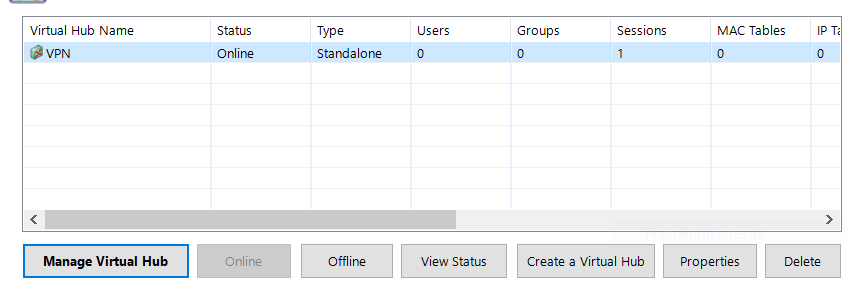
\includegraphics[width=0.6\textwidth]{SoftEther/korak13}
\end{figure}
\FloatBarrier
Sljedeći je korak odrediti tko se sve može povezati na naš server, a to se radi odabirom gumba ``Manage Virtual Hub''.
\begin{figure}[h!]
     \centering
     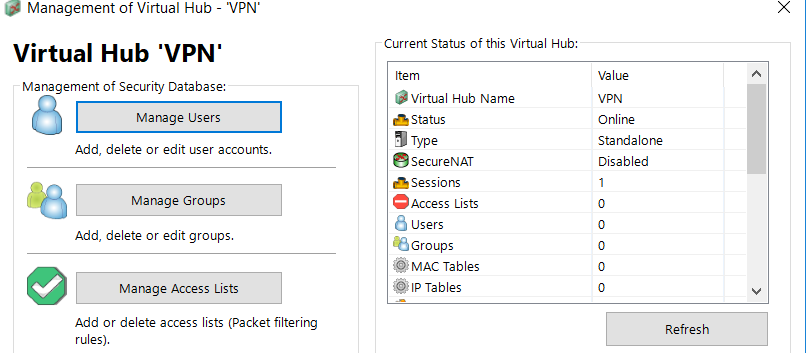
\includegraphics[width=0.6\textwidth]{SoftEther/korak14}
\end{figure}
\FloatBarrier
Na ovom prozoru odabiremo ``Manage Users''.
\begin{figure}[h!]
     \centering
     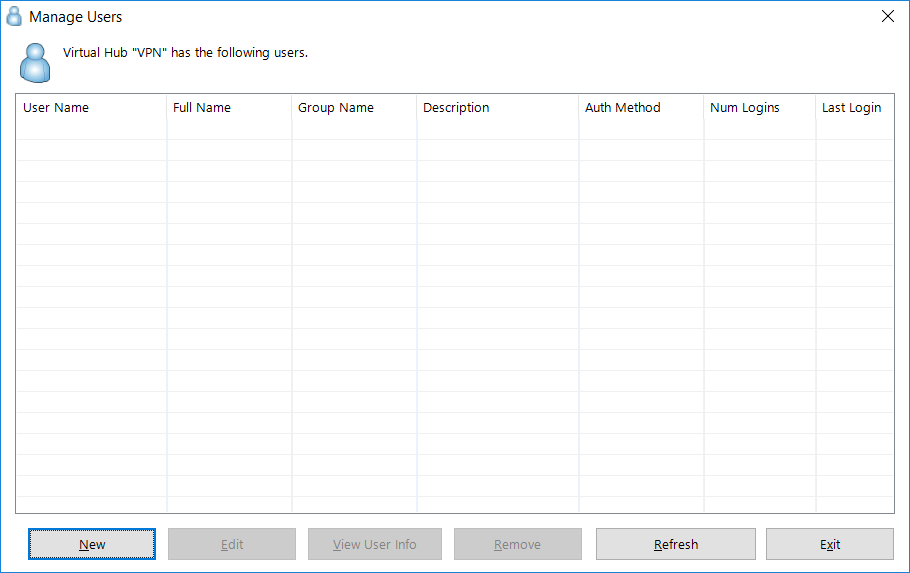
\includegraphics[width=0.4\textwidth]{SoftEther/korak15}
\end{figure}
\FloatBarrier
Sada dodajemo korisnika kojem ćemo dodati proizvoljno ime (u ovim je uputama korisnik nazvan ``klijent1'' i u svim narednim koracima gdje se to ime pojavljuje vama će se pojaviti vaše odabrano ime). Kako bismo smanjili vjerojatnost zlouporabe VPN-a, odabiremo mogućnost prijave klijenta uporabom našeg certifikata i lozinke. Zbog toga odabiremo ``Create Certificate''.
\begin{figure}[h!]
     \centering
     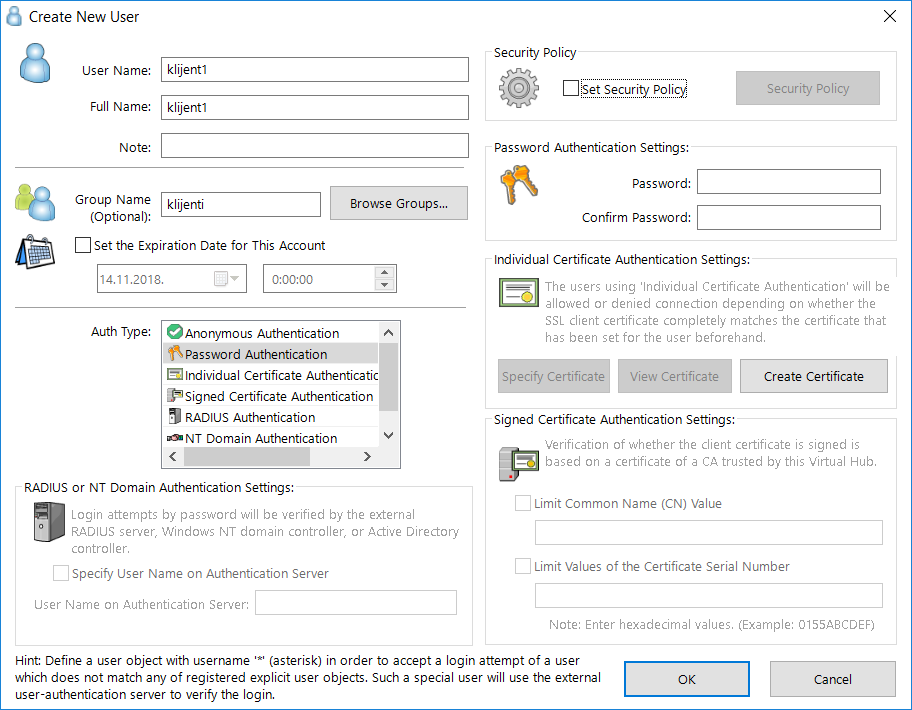
\includegraphics[width=0.6\textwidth]{SoftEther/korak16}
\end{figure}
\FloatBarrier
U sljedećim je poljima moguće detaljno odrediti opis stvorenog klijenta kao i vrijeme njegovog postojanja.
\begin{figure}[h!]
     \centering
     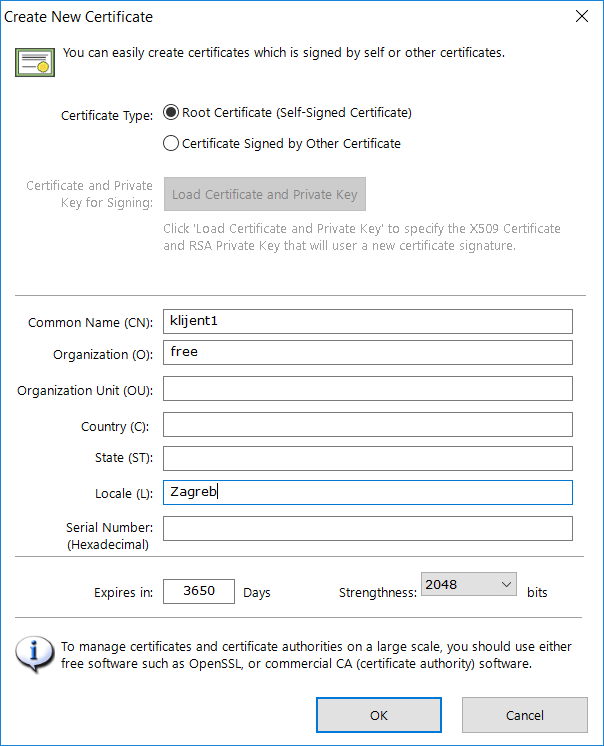
\includegraphics[width=0.6\textwidth]{SoftEther/korak17}
\end{figure}
\FloatBarrier
Nakon otvaranja ovog prozora postavljamo lozinku kojom će se naš klijent prijavljivati na server i koja će samo njemu biti poznata.
\begin{figure}[h!]
     \centering
     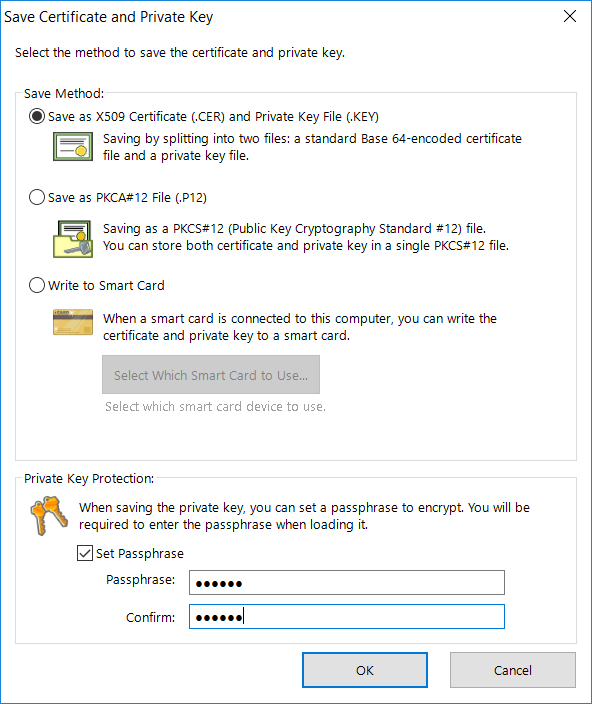
\includegraphics[width=0.6\textwidth]{SoftEther/korak18}
\end{figure}
\FloatBarrier
Nakon potvrde nastaju dvije datoteke: jedna je .cer, a druga je .key i obje su neophodne za prijavu na naš server zato ih mi moramo spremiti i prebaciti na računala koja će se htjeti povezati na server. Povezivanje na server objašnjeno je u jednom od sljedećih dijelova poglavlja.
\begin{figure}[h!]
     \centering
     
\includegraphics[width=0.3\textwidth]{SoftEther/korak20}
\end{figure}
\FloatBarrier
Nakon potvrde vidljiv je korisnik koji se može spojiti na naš server. Moguće je naravno dodavanje više različitih korisnika i brisanje istih.
\begin{figure}[h!]
     \centering
     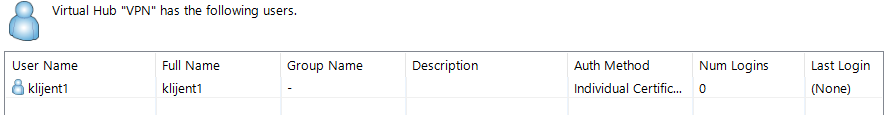
\includegraphics[width=0.6\textwidth]{SoftEther/korak19}
\end{figure}
\FloatBarrier

\newpage
\subsection*{Instalacija SoftEther klijenta}
\hspace{0.5cm}
Za razliku od instalacije i konfiguracije servera, instalacija je SoftEther klijenta jednostavnija. Prvi je korak preuzimanje instalacije sa službene stranice SoftEthera:\\ \url{https://www.softether.org}
\begin{figure}[h!]
	\centering
     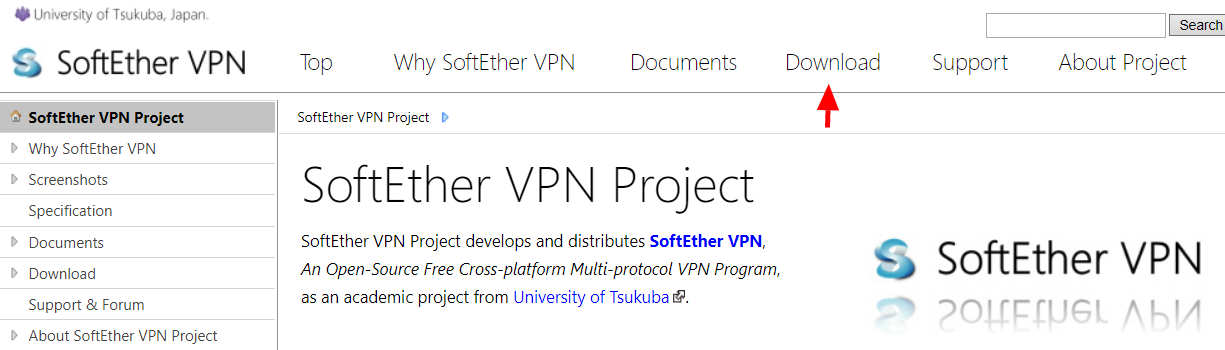
\includegraphics[width=0.6\textwidth]{SoftEther/korak1}
\end{figure}
\FloatBarrier
Odabirom ``Download'' iz izborne trake prikazuje se stranica s ponuđenim poveznicama za preuzimanje.
\begin{figure}[h!]
     \centering
     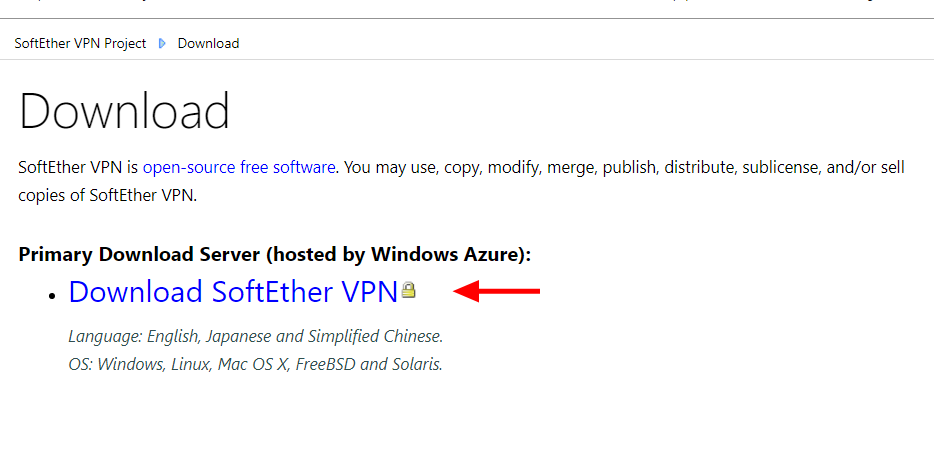
\includegraphics[width=0.6\textwidth]{SoftEther/korak2}
\end{figure}
\FloatBarrier
Sljedeći isječak prikazuje stranicu koja se otvori odabirom prve poveznice. Na stranici se nalaze izborni okviri u kojima je potrebno odabrati željeni program. Za preuzimanje VPN klijenta potrebno je odabrati postavke prikazane na sljedećem isječku te odabrati prvu poveznicu za početak preuzimanja.
\begin{figure}[h!]
     \centering
     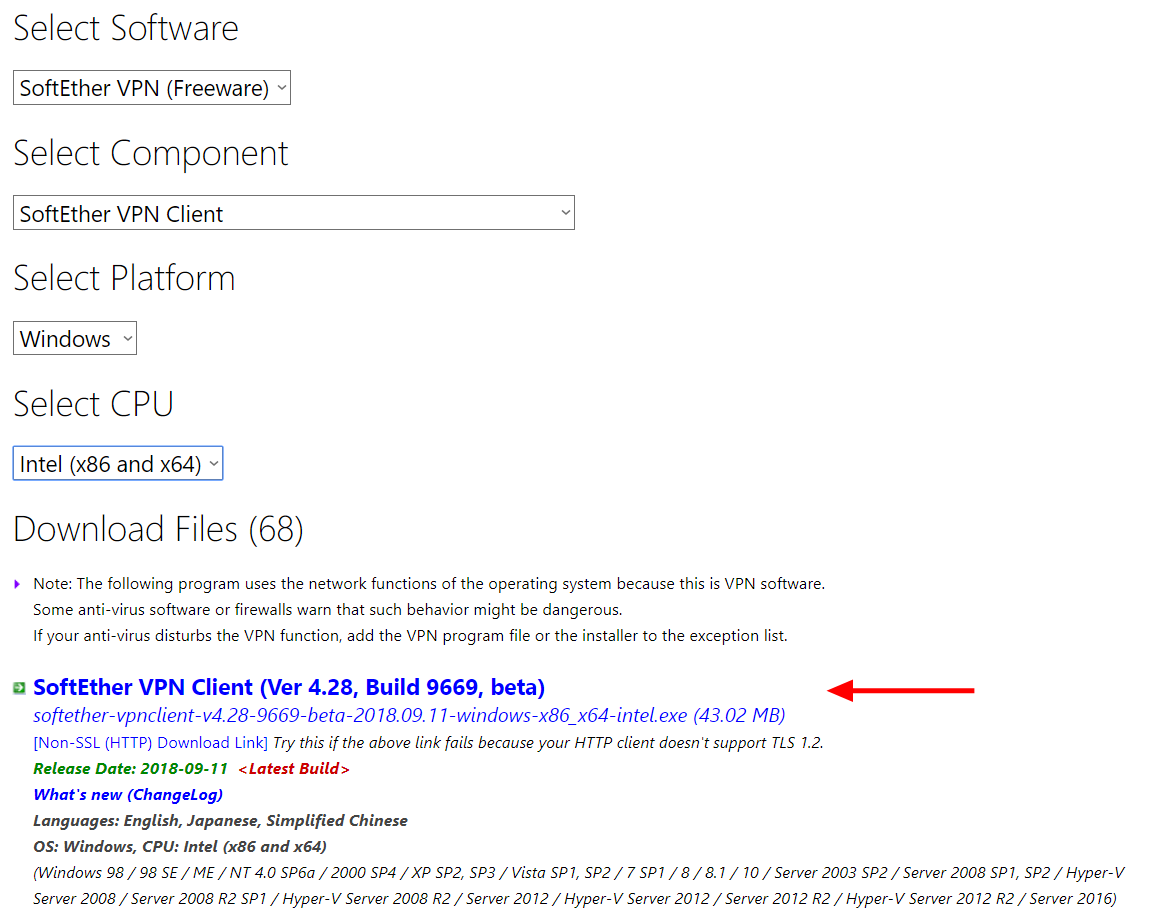
\includegraphics[width=0.6\textwidth]{SoftEther/korak3}
\end{figure}
\FloatBarrier
Nakon završetka preuzimanja i pokretanja instalacije prikazuje se sljedeći prozor. Preporuka je odabrati prvo ponuđeno jer nudi potpunu instalaciju programa.
\begin{figure}[h!]
     \centering
     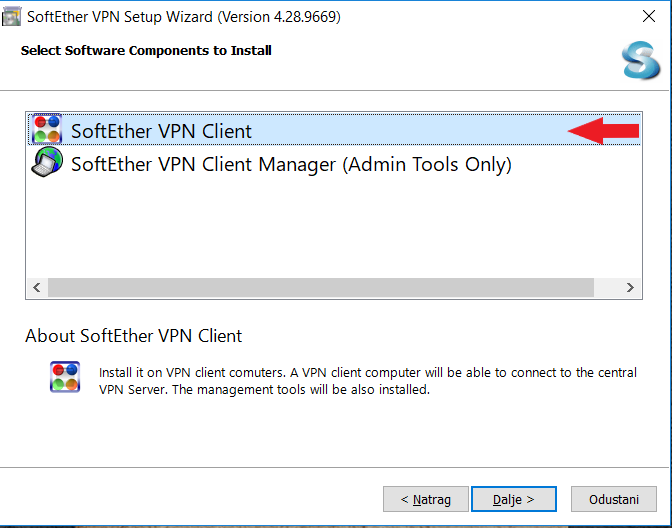
\includegraphics[width=0.6\textwidth]{SoftEther/korak4}
\end{figure}
\FloatBarrier
Ukoliko je instalacija uspješno završena, prikazuje se sljedeći prozor.
\begin{figure}[h!]
     \centering
     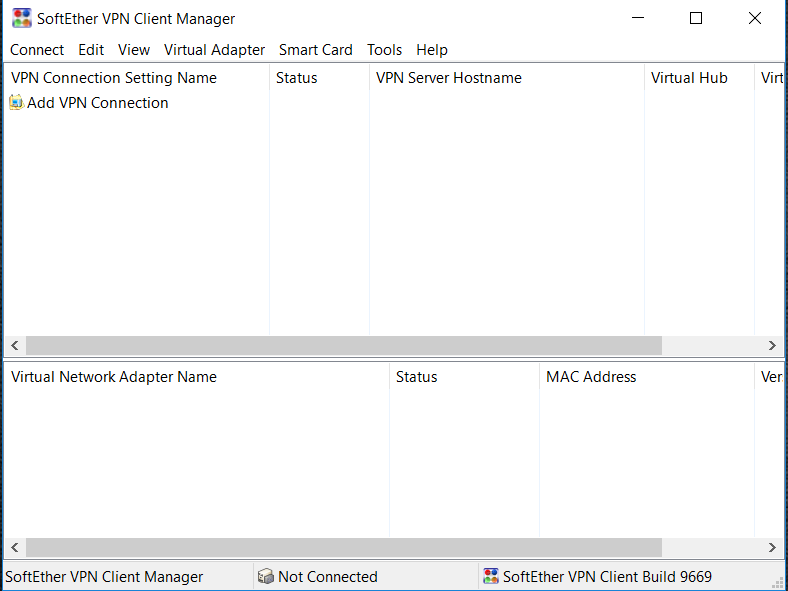
\includegraphics[width=0.6\textwidth]{SoftEther/korak5}
\end{figure}
\FloatBarrier

\newpage
\subsection*{Povezivanje klijenta sa SoftEther serverom}
\hspace{0.5cm}
Za uspješno povezivanje s napravljenim serverom potrebno je pokrenuti aplikaciju SoftEether VPN Client i odabrati opciju dodavanja novog VPN-a. Ako nije postavljen virtualni mrežni adapter, kao što je prikazano u sljedećem primjeru, potrebno je stvoriti novi. Prikazano je stvaranje VPN adaptera.
\begin{figure}[h!]
     \centering
     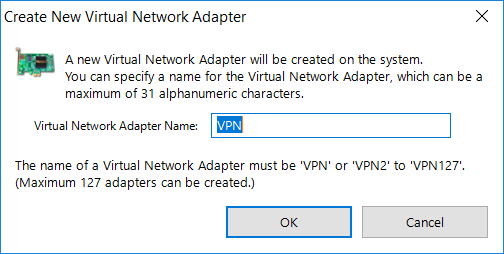
\includegraphics[width=0.6\textwidth]{SoftEther/korak21}
\end{figure}
\FloatBarrier
Nakon stvaranja adaptera moramo dodati server na koji se želimo povezati. Na slici je prikazano stvaranje veze koja se zove VPN. Slično kao i kod stvaranja servera, potrebno je upisati IP adresu preko koje se može serveru pristupiti u polje ``Host name''. Aplikacija nakon upisa IP adrese dohvaća portove na koje se moguće spojiti. Izbor je nekog od ponuđenih portova proizvoljan, kao i postojećih virtualnih mrežnih adaptera. Budući da smo prilikom stvaranja korisnika servera odabrali da se on može prijaviti samo uporabom certifikata i pripadnog ključa, potrebno je stvorene datoteke ``klijent1.cer'' i ``klijent1.key'' prebaciti na računalo s kojeg se pokušava povezati na server. Učitavanje certifikata i ključa u aplikaciju obavlja se odabirom opcije ``specify client certificate''.
\begin{figure}[h!]
     \centering
     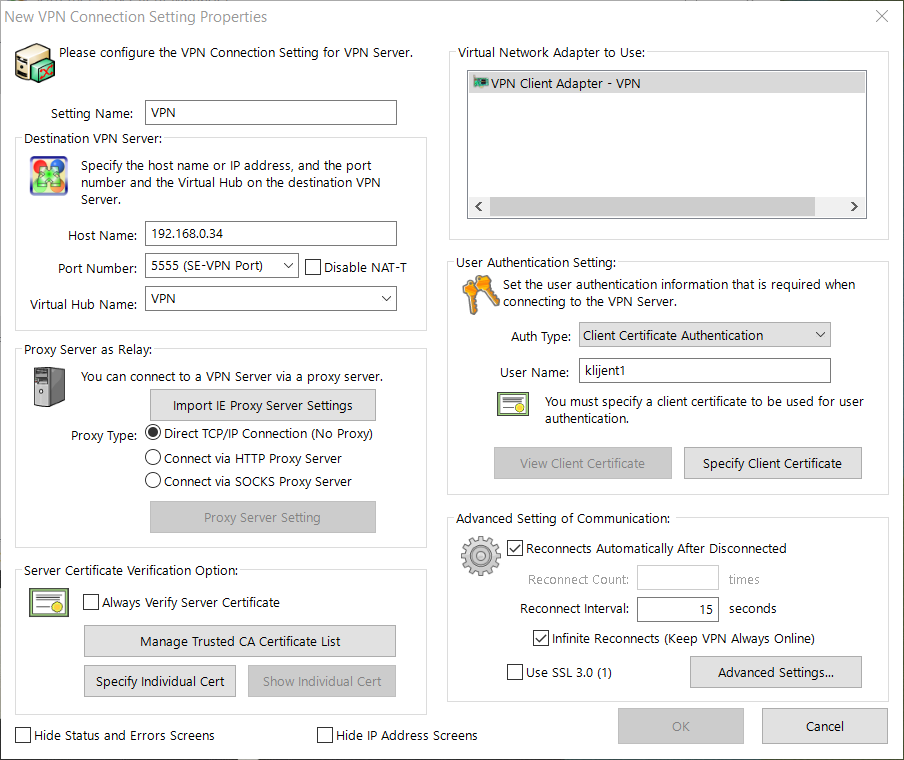
\includegraphics[width=0.6\textwidth]{SoftEther/korak22}
\end{figure}
\FloatBarrier
Nakon učitavanja datoteka prikazuje se prozor sa sljedećeg isječka u koji se upisuje lozinka koju smo postavili prilikom stvaranja klijenta.
\begin{figure}[h!]
     \centering
     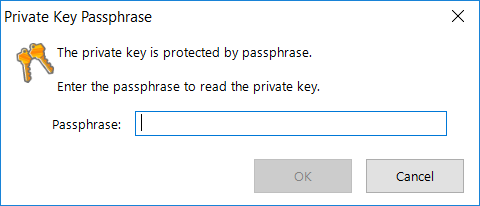
\includegraphics[width=0.6\textwidth]{SoftEther/korak23}
\end{figure}
\FloatBarrier
Ako smo učitali ispravni certifikat i unijeli ispravnu lozinku, tada će se prikazati prozor na kojem vidimo povezivanje s VPN serverom.
\begin{figure}[h!]
     \centering
     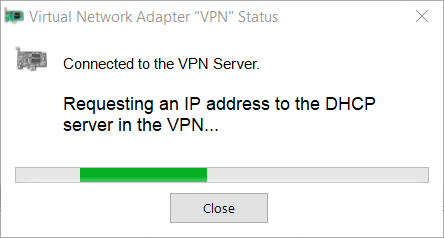
\includegraphics[width=0.5\textwidth]{SoftEther/korak24}
\end{figure}
\FloatBarrier

\FloatBarrier

\subsection*{Provjera vlastite IP adrese}
\hspace{0.5cm}
Kako bi server bio uspješno uspostavljen, potrebna mu je IP adresa dodijeljena računalu na kojem se nalazi. Najbrži način na koji se ona može odrediti jest otvaranje naredbenog retka i upis naredbe IPCONFIG. Rezultat te naredbe bit će prikaz mrežnih postavki za trenutno aktivne mrežne adaptere.
Crvenom je strelicom označena IP adresa na trenutno aktivnom adapteru.
\begin{figure}[h!]
     \centering
     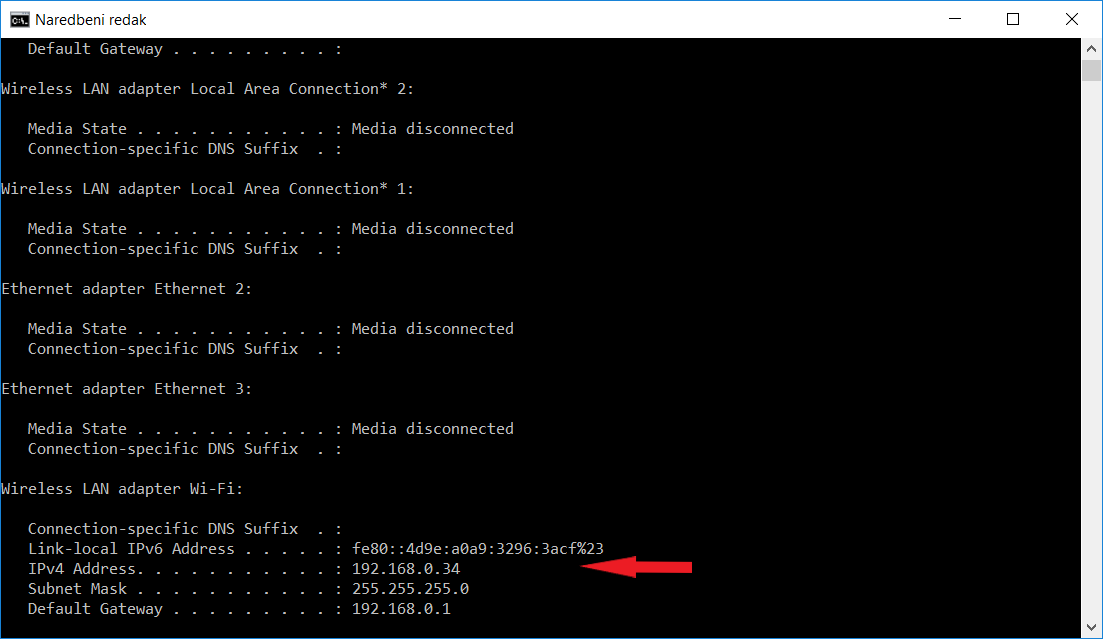
\includegraphics[width=0.6\textwidth]{SoftEther/IP1}
\end{figure}
\FloatBarrier

% za usporedbu === https://www.softether.org/@api/deki/files/12/=1.3.jpg
% pomoć pri instalaciji === https://www.youtube.com/watch?v=VbvRhPqNCsk